\section{Results}
\label{sec:results}
%Answer RQs and corresponding answers; 

%Reason where to put this segment/paragraph in the paper 

This section presents the results of our study, derived from analyzing the evidence extracted from the selected 41 studies and answering the defined RQs. It is worth noting that some interpretations may assume that the trends observed among the selected papers are indicative of broader publication patterns in the field.


\subsection{\textcolor{blue}{Descriptive analysis of included studies}}
\textcolor{blue}{We present here the trends pertaining to the publication space of the selected studies. The information regarding the venue name, venue type, publication year, and research area is tabulated in Table \ref{table:biblometric_analysis}. 
Despite not applying any restrictions on the publication date during the selection process, the earliest paper included in the analysis was published in 2005. Of the 41 selected papers, 31 (76\%) were published from 2021 onward, which indicates a growing interest in this topic in recent years. It is important to note that the low number of papers for 2025 is due to the fact that the paper extraction was carried out at the end of January; therefore, only papers published before this date were included.
Among the 41 selected papers, 28 were published in journals, and 13 in conference proceedings. 
The higher number of journal publications in the selected studies may be due to a higher likelihood of meeting the quality standards employed in this study.
With the exception of four publications in the journal ``Expert Systems with Application'', the remaining 37 studies were each published in a distinct venue.
In regards to the research areas of the publication venues, as expected for research on customer churn prediction using artificial intelligence, the dominant subject area associated with the publication venues of the selected studies was Computer Science with 29 studies, followed by Engineering with 19 studies, and subsequently by ``Mathematics, Physics, and Astronomy'' with 11 studies. ``Business, Economics, and Finance'' appeared in 7 studies, while Medicine and Neuroscience, Material Sciences, and the Multidisciplinary category were the least represented fields, with only 3, 2, and 1 associated studies, respectively. It is worth noting that each venue can be associated with multiple subject areas, meaning that the total number of subject-area associations exceeds the 41 selected studies.
Since not all conferences provide publicly available information on their subject areas, therefore, a procedure was adopted to ensure consistency in the analysis. The areas of interest for journal articles were obtained from Scimago\footnote{\url{https://www.scimagojr.com}}. For conferences lacking this information, the corresponding subject areas were retrieved from Scopus\footnote{\url{https://www.scopus.com}}.}

\begin{figure}[!htbp]
    \centering
    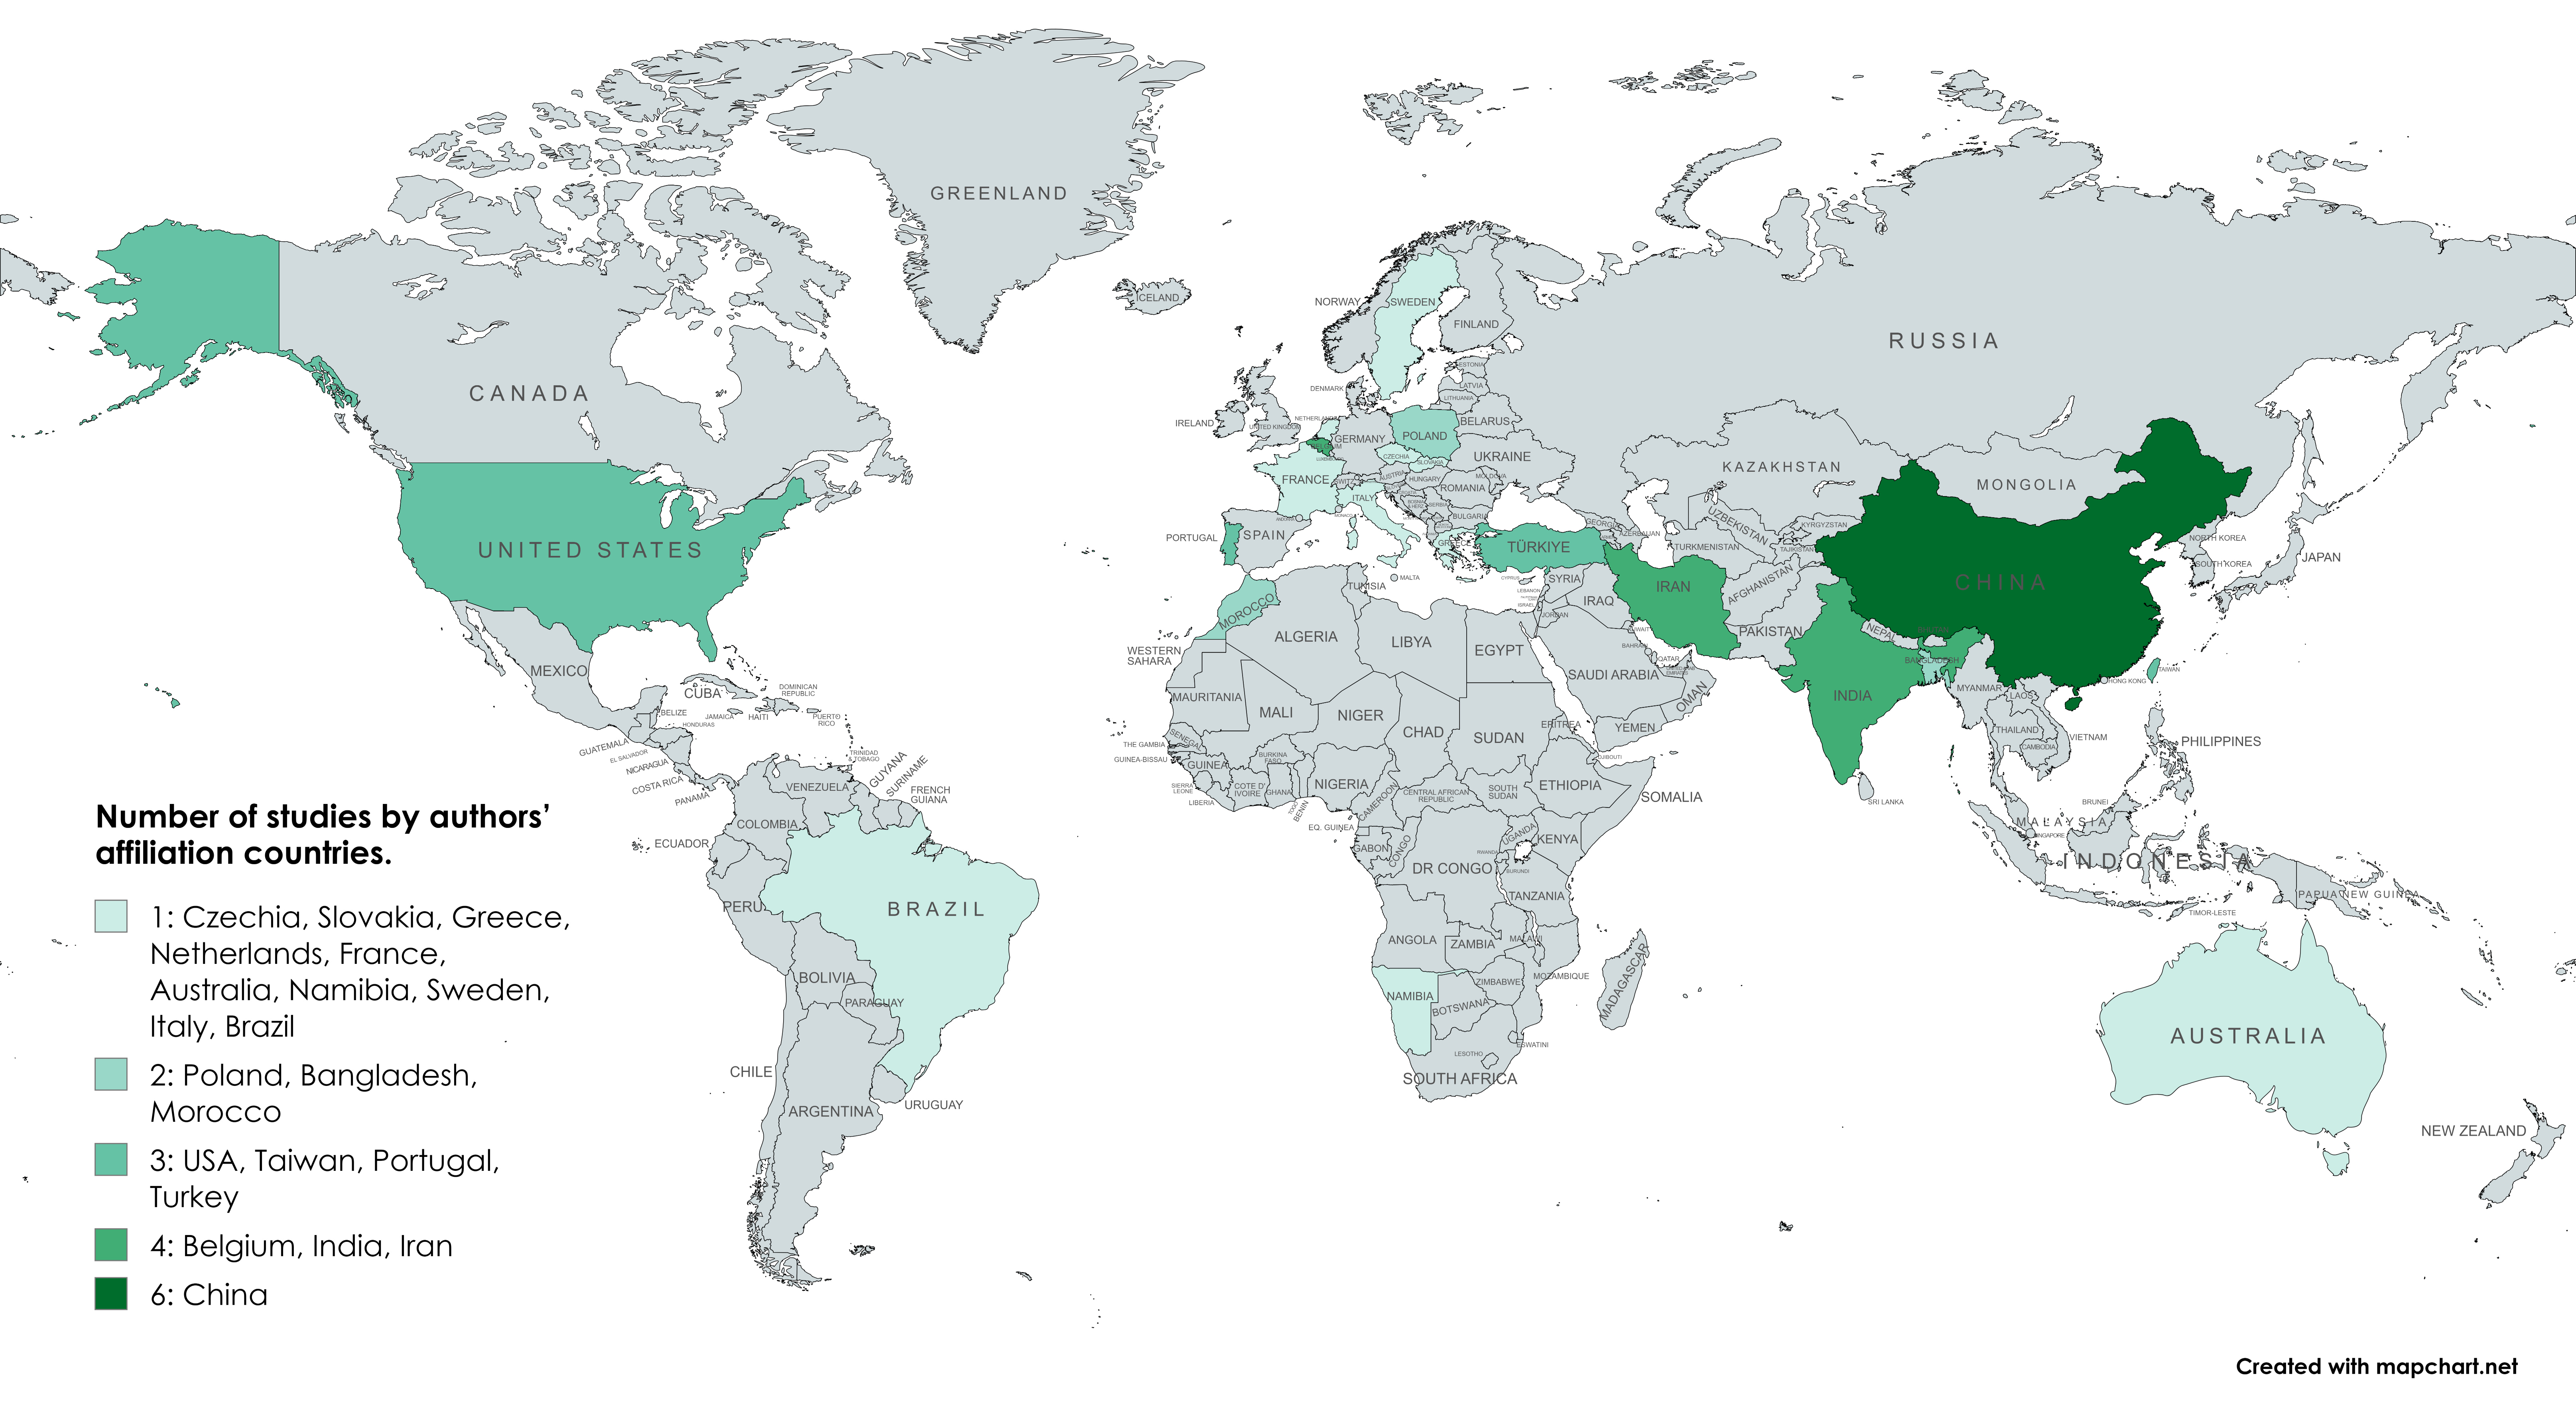
\includegraphics[width=\textwidth]{images/4_RESULTS/PS_RQ3_affiliation_countries.png}
    \caption{Distribution of selected studies by country of affiliation of authors.}
    \label{fig:PS_RQ3_Affiliation_Countries_Map}
\end{figure}    


 \textcolor{blue}{Figure \ref{fig:PS_RQ3_Affiliation_Countries_Map} presents the results of the author's affiliated country. Each country is counted only once per study, regardless of the number of authors affiliated with that country. If a study has authors from multiple countries, it is assigned to each of those countries. China had the highest representation, with six associated publications, followed by India, Belgium, and Iran, each contributing four publications. The United States, Taiwan, Portugal, and Turkey, each with three associated publications. Bangladesh, Morocco, and Poland contributed two publications each, while the remaining 10 countries were represented by a single publication.
It is worth noting that most publications originate from Asia, highlighting the region's particularly strong interest in the topic.}

\textcolor{orange}{Table \ref{tab:descriptive-summary} summarizes the main descriptive findings of the included studies.}

\begin{table}[H]
    \centering
    \caption{\textcolor{blue}{Summary of the main descriptive findings of the included studies}}
    \label{tab:descriptive-summary}
    \scriptsize
    \renewcommand{\arraystretch}{1.15}
    \begin{tabular}{|>{\raggedright\arraybackslash}p{0.18\textwidth}|>{\raggedright\arraybackslash}p{0.57\textwidth}|>{\raggedright\arraybackslash}p{0.17\textwidth}|}
        \hline
        \rowcolor{lightgray}
        \textbf{Topic} & \textbf{Finding} & \textbf{Reference} \\ \hline
        Publication trend & The earliest included study was published in 2005, and 31 of the 41 selected studies (76\%) were published from 2021 onward. & Table~\ref{table:biblometric_analysis} \\ \hline
        Venue type & Of the 41 selected studies, 28 were journal papers and 13 were conference papers. & Table~\ref{table:biblometric_analysis} \\ \hline
        Venue concentration & With the exception of four papers published in \textit{Expert Systems with Applications}, the remaining studies were distributed across distinct venues. & Table~\ref{table:biblometric_analysis} \\ \hline
        Research areas & Computer Science was the most represented research area (29 studies), followed by Engineering (19) and Mathematics, Physics, and Astronomy (11). & Table~\ref{table:biblometric_analysis} \\ \hline
        Geographic distribution & China had the highest representation with six associated publications, followed by India, Belgium, and Iran with four each. Most publications originated from Asia. & Figure~\ref{fig:PS_RQ3_Affiliation_Countries_Map} \\ \hline
    \end{tabular}
\end{table}


\begin{table}[H]
    \centering
    \caption{\textcolor{blue}{Bibliometrics of the included studies}}
    \label{table:biblometric_analysis}
    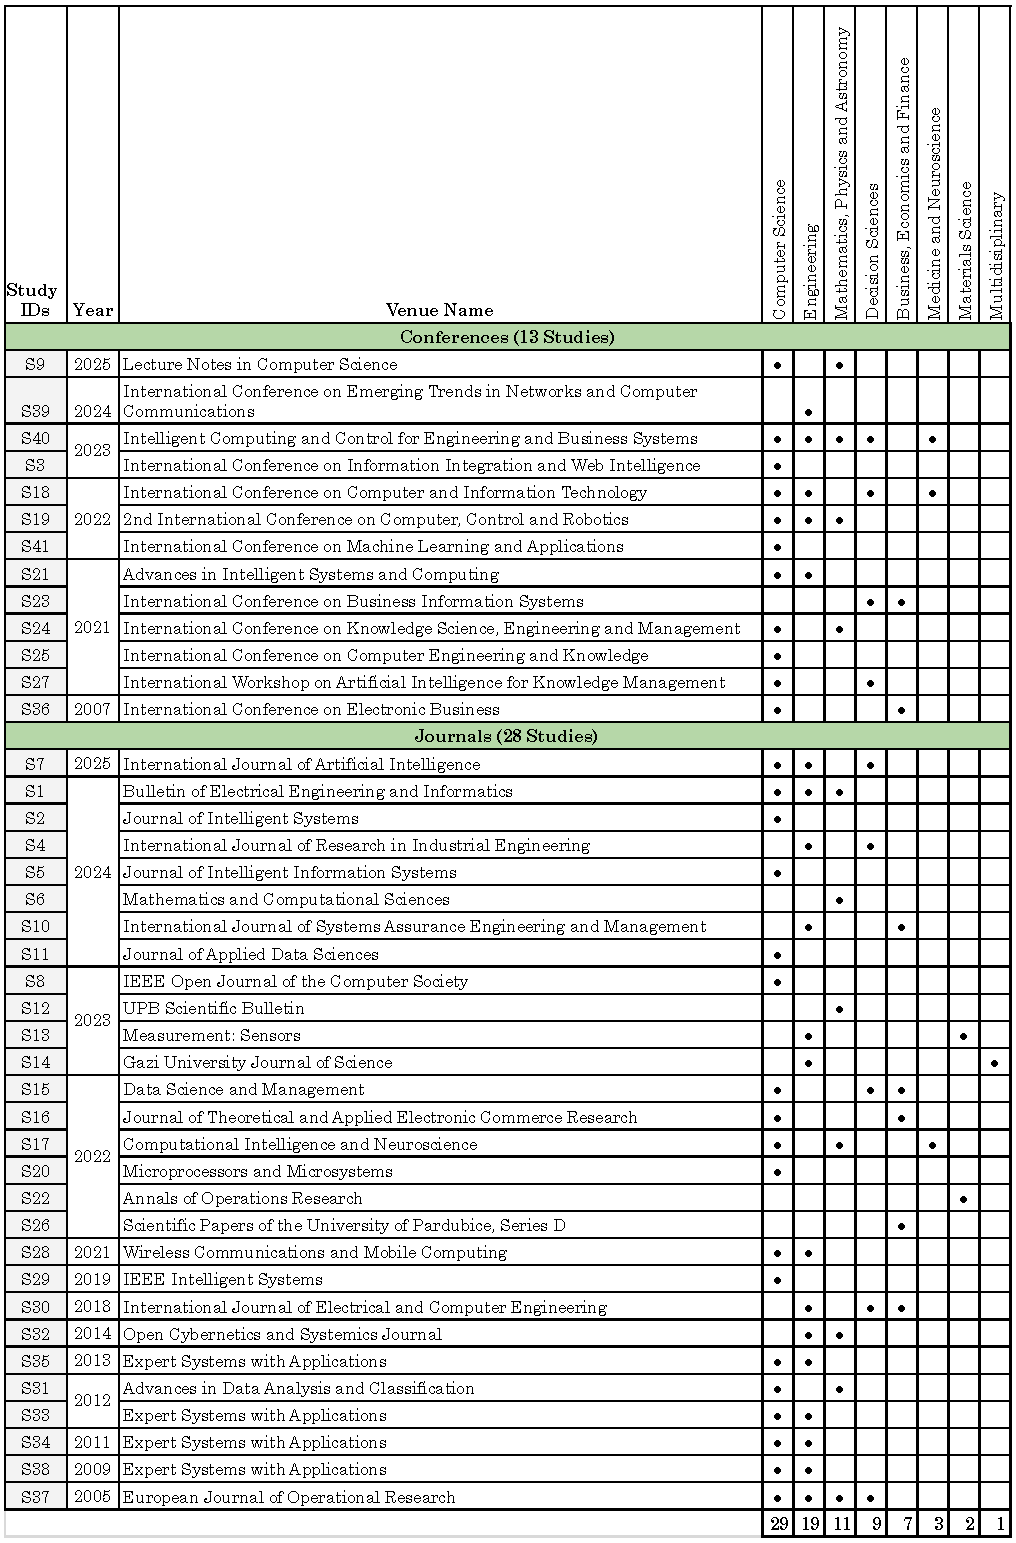
\includegraphics[width=0.91\textwidth]{pdf_tables/results/Bibliometrics_analysis.pdf}
\end{table}


\begin{comment}
\subsection{Answers to Publication Space Research Questions (PS-RQs)}
\subsubsection{\PSRQone}
%How are the selected studies distributed by publication year and venue type?

%proceed with the result and then insert the fact that there were no restrictions placed
No restrictions were applied to the publication date during the selection process of the primary studies. However, the earliest paper included in the analysis was published in 2005. As shown in Figure \ref{fig:PS_RQ1_venue_trend}, of the 41 selected papers, 31 (76\%) were published from 2021 onward, indicating a growing interest in this topic in recent years. It is important to note that the low number of papers for 2025 is due to the fact that the paper extraction was carried out at the end of January; therefore, only papers published before this date were included.
Among the 41 selected papers, 28 were published in journals, and 13 in conference proceedings (see Figure \ref{fig:PS_RQ1_pie_chart}). 
%Before applying the quality criteria, the distribution between journal and conference publications was more balanced. This shift suggests that journal publications were more likely to meet the quality standards employed in this study.
This distribution highlights a clear preference for journal publications, which may reflect their higher likelihood of meeting the quality standards employed in this study.

%TODO: Make the year of the graph more readable


\begin{figure}[h!]
    \centering
    \begin{subfigure}{0.48\textwidth}
        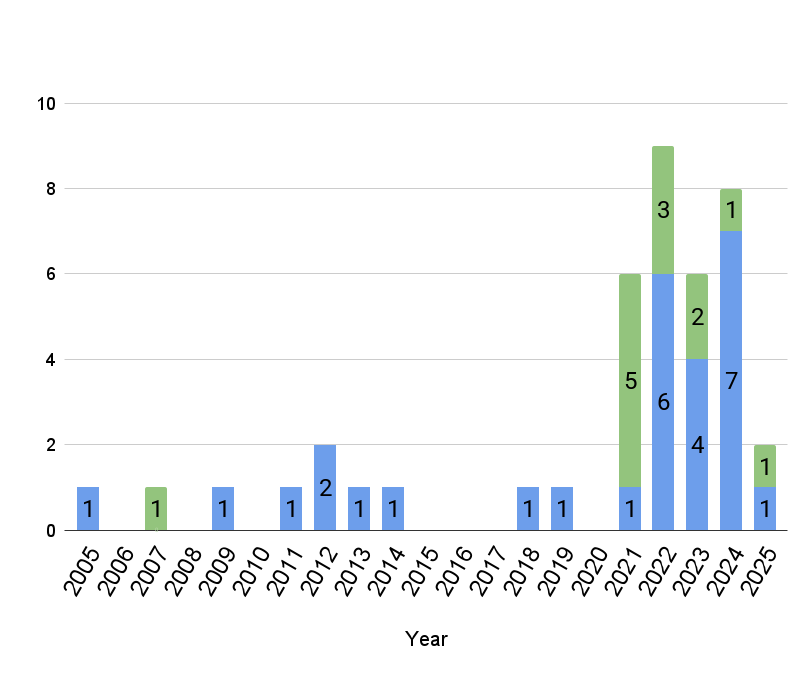
\includegraphics[width=\linewidth]{images/4_RESULTS/PS_RQ1_venue_trend.png}
        \caption{}
        \label{fig:PS_RQ1_venue_trend}
    \end{subfigure}   
    \hspace{0.02\textwidth}
    \begin{subfigure}{0.48\textwidth}
        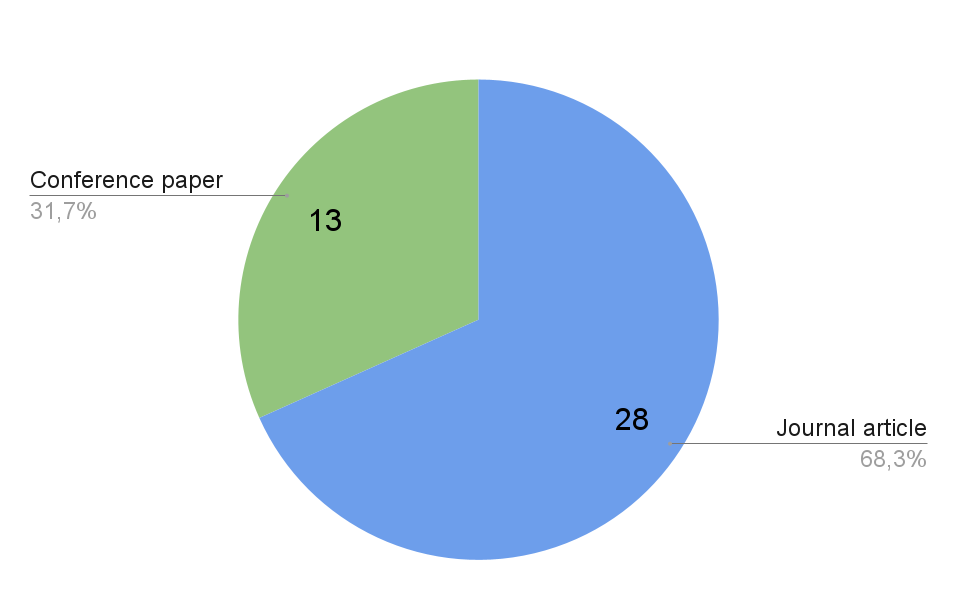
\includegraphics[width=\linewidth]{images/4_RESULTS/PS_RQ1_venue_pie_chart.png}
        \vspace{0.06\textwidth}
        \caption{}
        \label{fig:PS_RQ1_pie_chart}
    \end{subfigure}  
    \caption{Distribution of selected studies by publication year (a) and venue type (b).}
\end{figure}



\subsubsection{\PSRQtwo}

Table \ref{table:PS_RQ2_venues} presents the various publication venues of the 41 studies included in this analysis, along with the corresponding Study IDs for each venue. With the exception of four publications in the journal "Expert Systems with Application", the remaining 37 studies were each published in a distinct venue. Figure \ref{fig:PS_RQ2_research_area_distribution} illustrates the distribution of subject areas associated with the venues of all selected publications. 
As not all conferences provide publicly available information on their subject areas, a procedure was adopted to ensure consistency in the analysis. The areas of interest for journal articles were obtained from Scimago\footnote{\url{https://www.scimagojr.com}}. For conferences lacking this information, the corresponding subject areas were retrieved from Scopus\footnote{\url{https://www.scopus.com}}.

As expected for research on customer churn prediction using artificial intelligence, the dominant subject area associated with the publication venues of the selected studies was Computer Science with 29 studies, followed by Engineering with 19 studies, and subsequently by 'Mathematics, Physics, and Astronomy' with 11 studies. 'Business, Economics, and Finance' appeared in 7 studies, while Medicine and Neuroscience, Material Sciences, and the Multidisciplinary category were the least represented fields, with only 3, 2, and 1 associated studies, respectively. It is worth noting that each venue can be associated with multiple subject areas, meaning that the total number of subject-area associations exceeds the 41 selected studies.
%add numbers regarding the information provided (how many were on CS, etc) and provide the information first and then any comments (THIS IS VALID FOR ALL ANSWERS). (Done)

%Article -> Journal (Table) (Done)



\begin{table}[htbp]
\centering
\footnotesize
\renewcommand{\arraystretch}{1.1}
\caption{Study publication venues.}
\label{table:PS_RQ2_venues}
\resizebox{0.8\textwidth}{!}{
\begin{tabular}{|
  >{\raggedright\arraybackslash}m{12.5cm}
  |>{\centering\arraybackslash}m{2cm}|}
\hline
\rowcolor[HTML]{D5E8D4} 
\textbf{Venue Name} & \textbf{Study IDs} \\ \hline
\rowcolor{lightgray} 
\multicolumn{2}{|c|}{\textbf{Journals}} \\ \hline
Bulletin of Electrical Engineering and Informatics & S1 \\ \hline
Journal of Intelligent Systems & S2 \\ \hline
International Journal of Research in Industrial Engineering & S4 \\ \hline
Journal of Intelligent Information Systems & S5 \\ \hline
Mathematics and Computational Sciences & S6 \\ \hline
International Journal of Artificial Intelligence & S7 \\ \hline
IEEE Open Journal of the Computer Society & S8 \\ \hline
International Journal of Systems Assurance Engineering and Management & S10 \\ \hline
Journal of Applied Data Sciences & S11 \\ \hline
UPB Scientific Bulletin & S12 \\ \hline
Measurement: Sensors & S13 \\ \hline
Gazi University Journal of Science & S14 \\ \hline
Data Science and Management & S15 \\ \hline
Journal of Theoretical and Applied Electronic Commerce Research & S16 \\ \hline
Computational Intelligence and Neuroscience & S17 \\ \hline
Microprocessors and Microsystems & S20 \\ \hline
Annals of Operations Research & S22 \\ \hline
Scientific Papers of the University of Pardubice, Series D & S26 \\ \hline
Wireless Communications and Mobile Computing & S28\\ \hline
IEEE Intelligent Systems & S29 \\ \hline
International Journal of Electrical and Computer Engineering & S30 \\ \hline
Advances in Data Analysis and Classification & S31 \\ \hline
Open Cybernetics and Systemics Journal & S32 \\ \hline
Expert Systems with Applications & S33, S34, S35, S38 \\ \hline
European Journal of Operational Research & S37 \\ \hline
\rowcolor{lightgray} 
\multicolumn{2}{|c|}{\textbf{Conferences}} \\ \hline
International Conference on Information Integration and Web Intelligence & S3 \\ \hline
Lecture Notes in Computer Science & S9 \\ \hline
International Conference on Computer and Information Technology & S18 \\ \hline
International Conference on Computer, Control and Robotics & S19 \\ \hline
Advances in Intelligent Systems and Computing & S21 \\ \hline
International Conference on Business Information Systems & S23 \\ \hline
International Conference on Knowledge Science, Engineering and Management & S24 \\ \hline
International Conference on Computer Engineering and Knowledge & S25 \\ \hline
International Workshop on Artificial Intelligence for Knowledge Management & S27 \\ \hline
International Conference on Electronic Business & S36 \\ \hline
International Conference on Emerging Trends in Networks and Computer Communications & S39 \\ \hline
Intelligent Computing and Control for Engineering and Business Systems & S40 \\ \hline
International Conference on Machine Learning and Applications & S41 \\ \hline
\end{tabular}
}
\end{table} %now is left aligned




% Need to somehow reference the studies to they appear in the biblograpy 

\begin{figure}[h]
    \centering
    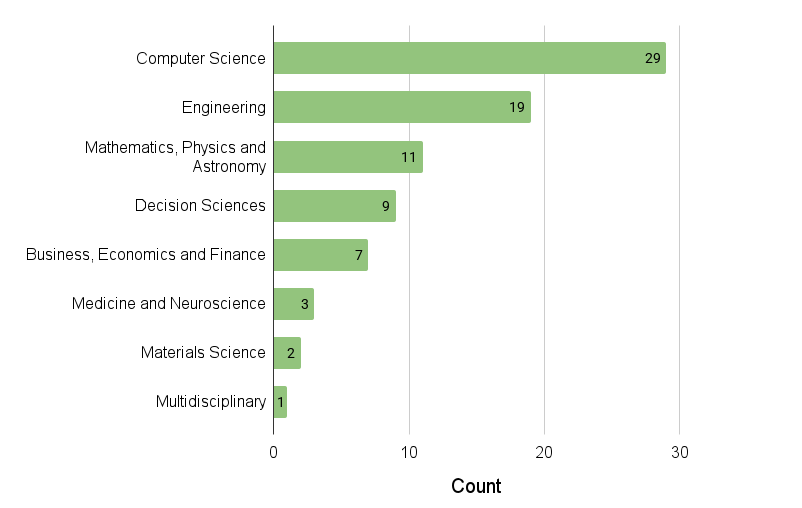
\includegraphics[width=0.8\textwidth]{images/4_RESULTS/PS_RQ2_research_area_distribution.png}
    \caption{Distribution of selected studies by research areas of the publication venues.}
    \label{fig:PS_RQ2_research_area_distribution}
\end{figure}  





\subsubsection{\PSRQthree}

%This section presents the affiliated countries for each publication. Each country is counted only once per study, regardless of the number of authors from that country. For example, if multiple authors in a single study are affiliated with the same country, it is counted as a single occurrence.

%Among the included studies, 12 were single-author publications, 36 studies had authors from the same country whereas 5 publications involved affiliations from two different countries. No study featured authors from more than two countries.



\end{comment}
%PRISMA Flowchart used for paper selection; Classification of each analyzed %paper; majority of Figures are added now.


\subsection{Answers to \textcolor{blue}{Research Questions (RQs)}}
%Tell about what we explain in this section. Give the definition, the number of papers that use it and why.


\subsubsection{\RSRQone}
\label{sec:RQ1}

In non-contractual settings such as Fast Moving Consumer Goods (FMCG) and e-commerce, defining churn presents a significant challenge. Unlike contractual industries, where customers formally terminate their relationship, churn in non-contractual sectors is a behavioral inference rather than a clearly observable event. Our review found that more than one-third of the 41 surveyed studies did not provide a clear definition of churn. In many cases, this omission was due to the use of pre-processed or third-party datasets, particularly those sourced from platforms such as Kaggle\footnote{\url{kaggle.com}}, where churn is provided as a pre-labeled flag with minimal or no documentation or behavioral context. Moreover, several studies relied on external datasets or cited sources that were either inaccessible or insufficiently described, rendering their churn definitions non-replicable. Even when a definition was provided, it was often vague or overly simplistic, lacking the detail necessary for methodological transparency and reproducibility.

%\begin{table}[H]
%    \centering
%    \caption{Churn Definition Groups.}
%    \label{fig:RS_RQ1_churn_definition}
%    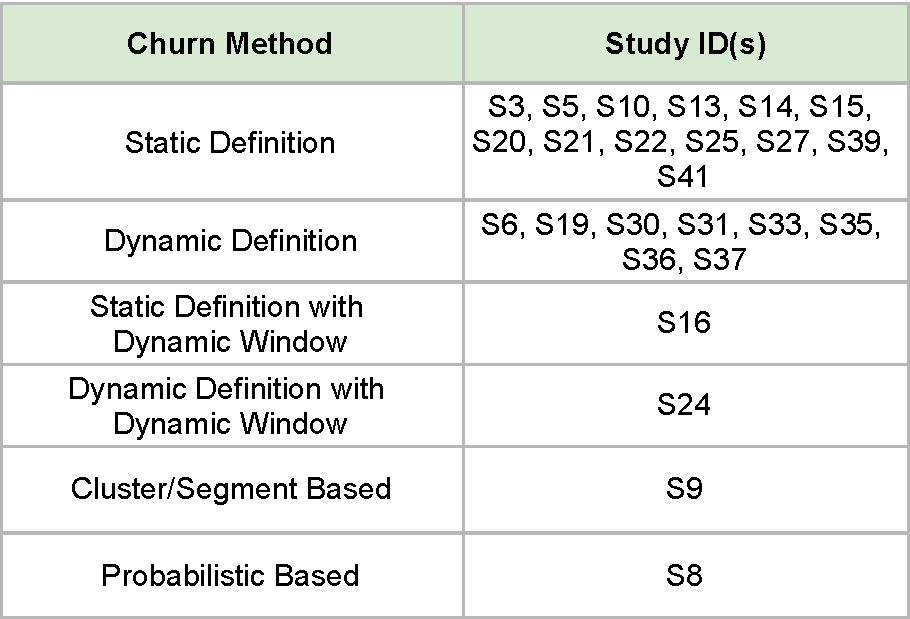
\includegraphics[width=.5\textwidth]{pdf_tables/results/RS_RQ1_churn_definition.pdf}
%\end{table}

\begin{table}[h]
    \caption{Adopted churn definitions and associated studies.}
    \label{tab:RS_RQ1_churn_definition}
    \centering
    %{\fontfamily{phv}\selectfont   % inizio gruppo → Helvetica/Arial-like
    \scriptsize                 % o \footnotesize, \small…
    \resizebox{0.7\textwidth}{!}{
    \begin{tabular}{|
  >{\centering\arraybackslash}m{4.5cm}
  |>{\centering\arraybackslash}m{5cm}|}
    \hline
    \rowcolor[HTML]{D5E8D4} 
    \rule[-1.5ex]{0pt}{4ex}\textbf{Churn definition}
  & \rule[-1.5ex]{0pt}{4ex}\textbf{Study ID(s)} \\ \hline
    Static & S3, S5, S10, S13, S14, S15, S20, S21, S22, S25, S27, S39, S41 \\ \hline
    Dynamic & S6, S19, S30, S31, S33, S35, S36, S37 \\ \hline
    Static with dynamic window & S16, S23 \\ \hline
    Dynamic with dynamic window & S24 \\ \hline
    Cluster/Segment based & S9 \\ \hline
    Probabilistic based & S8 \\ \hline
    \end{tabular}
    }
 % }% fine gruppo → torna al font normale qui
\end{table}


%We begin by describing the different categories as can be seen in Table \ref{tab:RS_RQ1_churn_definition} of churn prediction used in the selected studies.



\textcolor{blue}{To classify heterogeneous definitions in a consistent way, we conducted a thematic analysis of the churn definitions reported in the selected studies. To the best of our knowledge, no systematic typology of churn in non-contractual retail contexts exists.  Therefore, our analysis focuses on the operational definitions of churn used in practice rather than on new conceptual types of churn.
We used the data extraction form described in Section \ref{sec:methodology} to collect, for each study, the textual definition of churn and the details of its specifications.
We then iteratively coded each study along two main dimensions: \emph{i.} how the temporal window used to assess churn is defined (fixed length that is identical for all customers vs.\ implicitly or explicitly customer-specific), and \emph{ii.} how churn is determined within that window (fixed heuristic thresholds on inactivity or spending, behaviour-based thresholds relative to a reference period, or data-driven mechanisms such as clustering or probabilistic models). 
By systematically combining the values of these two dimensions and applying the resulting scheme to all 26 studies that provide an explicit operational definition of churn, we derived a data-driven taxonomy of six archetypal churn definitions. This taxonomy is summarized in Table~\ref{tab:RS_RQ1_churn_definition}, together with the associated Study IDs, and provides a unifying lens to map heterogeneous definitions found in the literature. Although it is grounded in our sample, the taxonomy is general enough to be used as a reference framework in future research on churn prediction in non-contractual retail environments.
The following categories of churn definitions were identified:}


\begin{itemize}
    \item \textit{Static definition}: This is the most common and straightforward approach. Churn is defined based on a fixed window period (e.g., 90 days, 3 months, or 1 year) during which the absence or reduction of customer activity is interpreted as churn. The threshold (e.g., no spending or a significant drop in purchases) is applied uniformly across all customers, regardless of their behavioral patterns. While this method is easy to implement and interpret, it lacks personalization and may overlook individual variations in engagement.
    
    \item \textit{Dynamic definition}: This method employs fixed-length observation and labeling windows (e.g., P1 = 3 months, P2 = 3 months). Churn is identified based on significant changes in customer behavior between these two periods. For example, a customer is labeled as churned if their loyalty in P2 declines sharply compared to their behavior during P1, or if their spending in P2 falls below a threshold that is behaviorally derived from P1. This approach captures behavioral shifts and partial churn more effectively than static definitions.
    
    \item \textit{Static definition with dynamic window}: 
    %Churn is assessed using a dynamic observation window defined by an event, such as the absence of subsequent purchases. However, the threshold for labeling churn within this window, for example using criteria like no further purchases or no activity beyond a predefined duration, remains fixed. This approach introduces some adaptability in identifying the observation period while preserving the simplicity of a static threshold.
    This approach evaluates churn based on an observation window whose start and/or length are dynamically determined by an event specific to the customer's purchase history (e.g., the customer's first or most recent transaction), while the threshold used to label churn (e.g., no purchases) remains static and uniformly applied to all customers.
    This approach introduces some adaptability in identifying the observation period while preserving the simplicity of a static threshold.
    
    \item \textit{Dynamic definition with dynamic window}: This is the most flexible and personalized approach. Both the observation window and the churn threshold are determined based on each customer’s unique behavioral history. For example, the window start point can be determined by their second last purchase and the dynamic recency threshold for churn can be determined for each customer as a multiple of their last two transactions.. This fully dynamic strategy enables highly tailored churn definitions and is commonly adopted in advanced models that prioritize precision over simplicity.

    \item \textit{Cluster/segment-based}: In this category, churn is inferred through data-driven segmentation techniques, such as K-means clustering, which group customers based on behavioral patterns. Customers assigned to groups exhibiting a complete absence or substantial reduction of activity are labeled as churners. This unsupervised approach does not rely on predefined thresholds, but rather identifies churn through emergent patterns in the data. Only one study employed this definition.
     
    \item \textit{Probabilistic-based}: This approach uses statistical or machine learning models to estimate the probability that a customer remains active. When this probability falls below a predefined threshold, the customer is classified as a churner. This method allows for dynamic adjustment based on differing consumption patterns and cycles. Among the reviewed studies, only one adopted this method.

\end{itemize}

%TODO: once this part is checked and the extraction is finalized, add a final sentence to state the level of the definitions provided


It is interesting to note that this simple approach dominates the literature with 13 studies using this method. This is followed by the dynamic definition method, which is utilized by 9 studies. The static definition with dynamic window approach is used by 2 studies. The other more bespoke approaches, including probabilistic and segmentation methods, are utilized only by one study.

\subsubsection{\RSRQtwo}
\label{sec:RQ2}
The analysis of the 41 selected studies revealed a wide range of features employed for customer churn prediction,  with some proving particularly effective in capturing churn-related behavior. Due to inconsistent terminology used across studies, feature names were standardized where possible to enable consistent comparison. When only intermediary or derived variables were reported, they were traced back and mapped to their most likely source features to align with a common feature taxonomy.

Variables such as \textit{Customer ID}, \textit{Transaction ID}, and other similar identifiers were excluded, as they do not provide meaningful information for churn prediction. These variables are primarily used within the data processing pipeline to consolidate records at the customer level.

The top section of Table \ref{table:RS_RQ2_features} lists the features used for churn prediction across the selected studies, indicating for each study whether they were used and, if applicable, whether they were identified as top features.
Empty circles (\textopenbullet) denote intermediary or derived variables, while filled circles (\textbullet) mark features explicitly identified as most important in the studies. Columns corresponding to studies with unclear source features are shaded in light grey.

%In cases where the available information was not sufficient to identify the original source features, the corresponding study row is shaded in light grey. When such information is available, the feature is indicated with an empty circle symbol (\textopenbullet). 
%If the study explicitly assessed the contribution of individual features to predictive performance, the best features identified by the study are then marked by a filled circle (\textbullet). 
The bottom section summarizes the use of feature categories. Each category is marked for a study if at least one variable from that category was included in the study. For studies in which the source features could not be fully identified but enough details were available to determine usage at the category level, only the relevant categories are indicated. These columns are also shaded in grey.
%We now describe the six feature categories identified, offering insights into each category. 

\textbf{\begin{table}[t]
    \centering
    \caption{Features used for churn prediction, with top-ranked features highlighted.
    %\DD{}{Consider highlighting in the table, e.g., with a round rectangle overlapping it, rows associated features common to most studies/datasets, and rows associated to best predicting features]}
    }
    \label{table:RS_RQ2_features}
    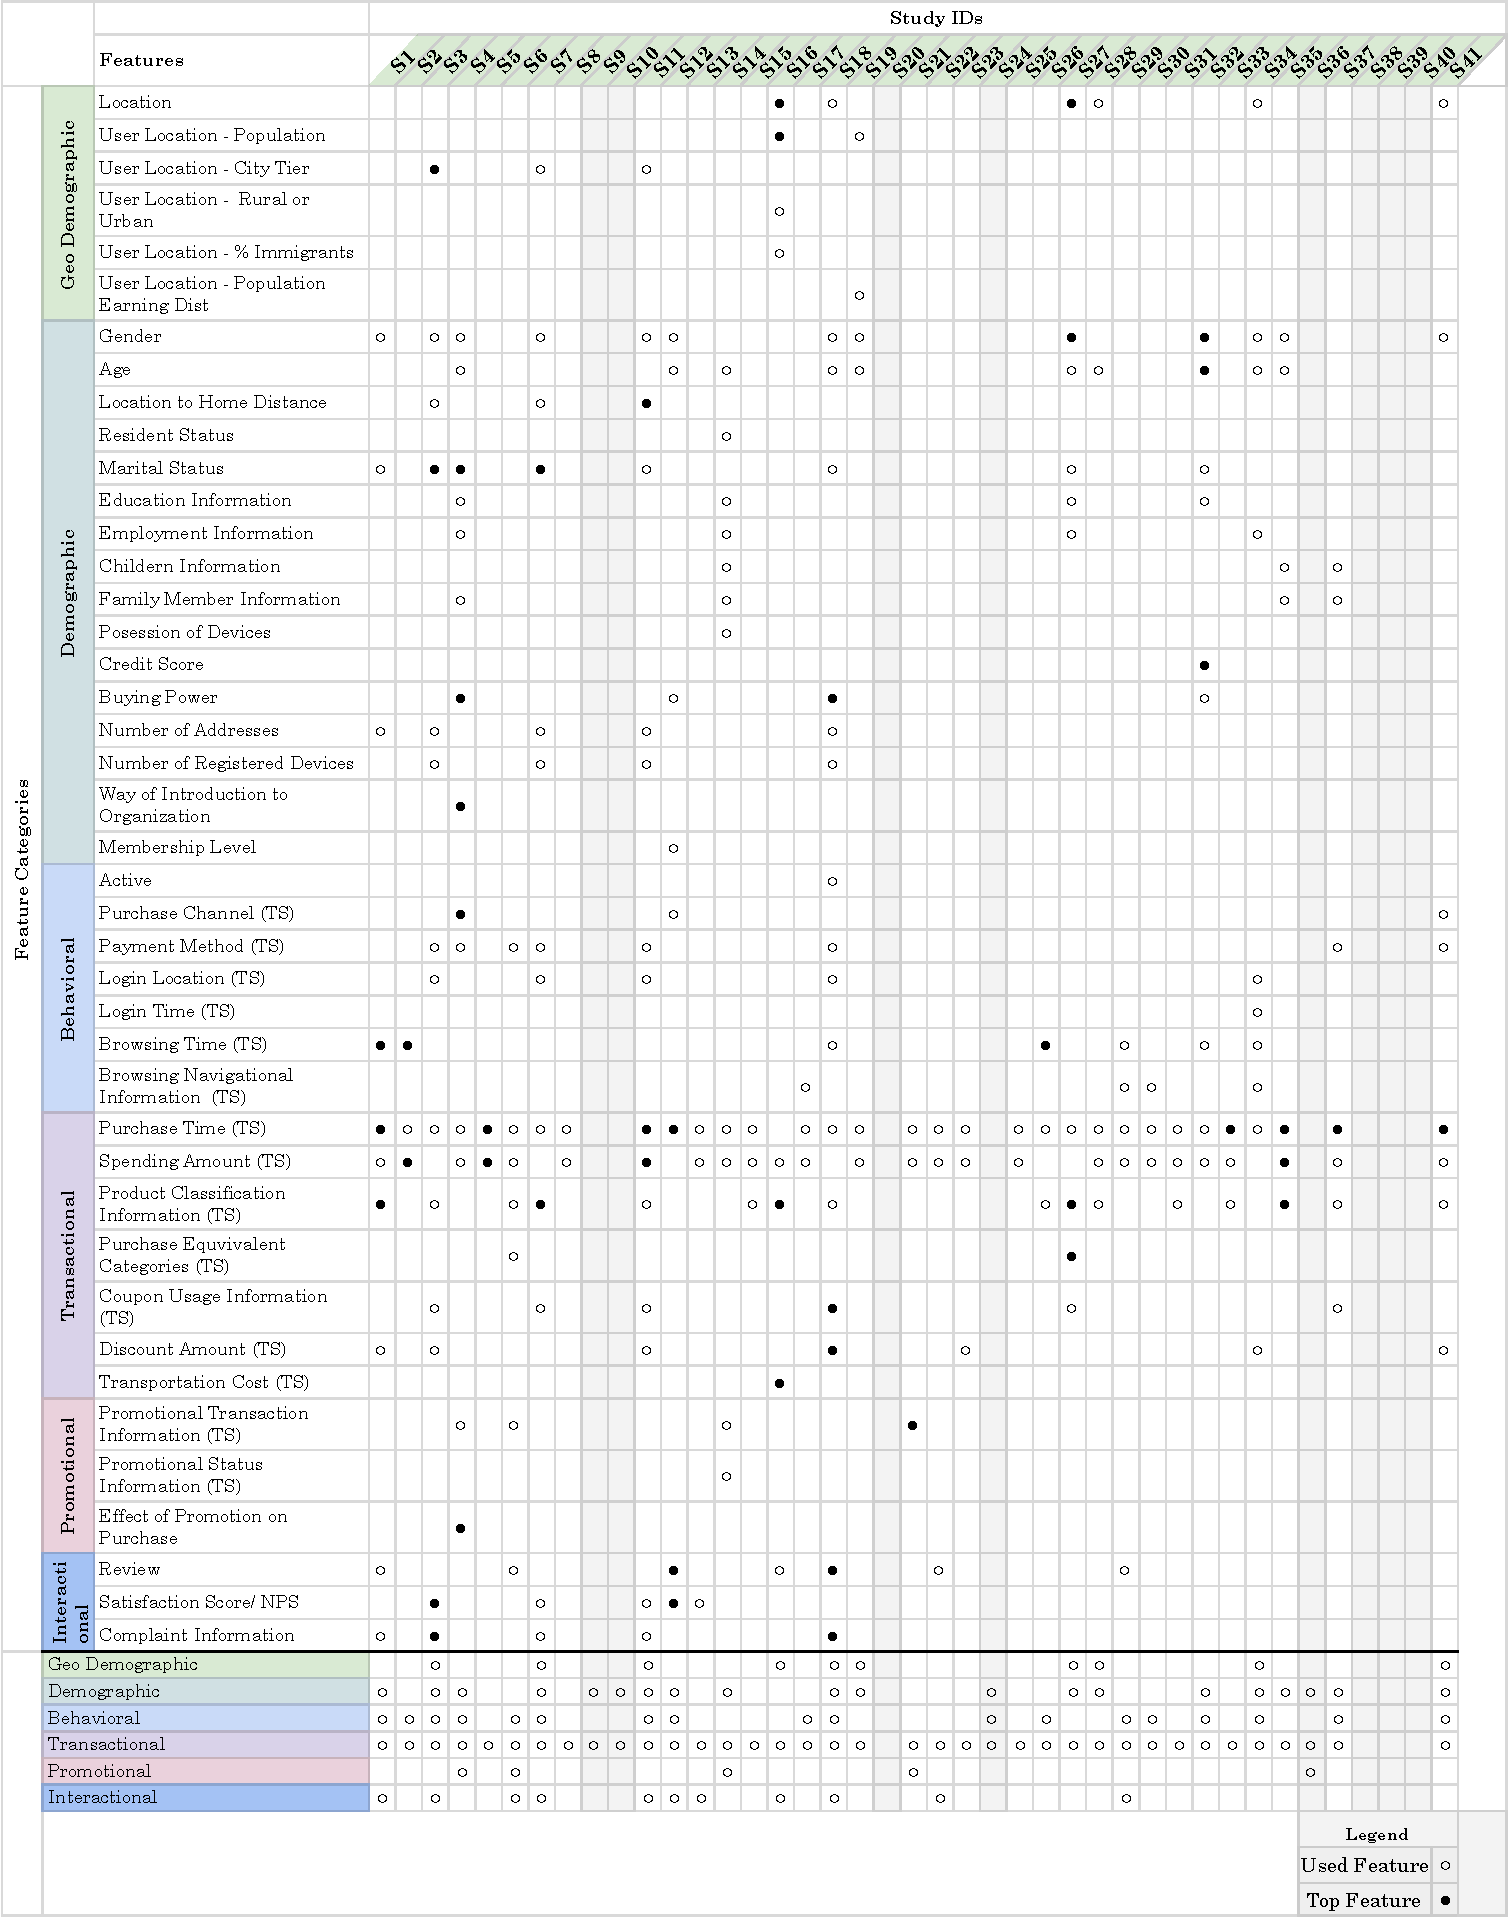
\includegraphics[width=\textwidth]{pdf_tables/results/RS_RQ2_features.pdf}
\end{table}}
\FloatBarrier

Subsequently, we present our observations regarding the specific features employed in the selected studies, with particular attention to those identified as most effective for churn prediction. 
%Overall, the features used can be broadly grouped into six main categories:


\begin{enumerate} 
\item \textit{Geo-demographic:}
Features belonging to this category capture the demographic characteristics of the customer's location (e.g., population density, income levels, economic activity, neighborhood composition), rather than the customer's personal attributes. %Examples include local population density, average income levels, regional economic activity, and neighborhood composition. 
While indirect, these features can provide useful contextual signals for customer behavior.

\item \textit{Demographic:}
This category includes personal demographic details of the customer, such as gender, age, marital status, occupation, and education level. These features are typically available early in the customer lifecycle and can aid in early-stage churn prediction.

\item \textit{Behavioral:}
Behavioral features capture how customers interact with the business outside of transactions. In e-commerce settings, this may include browsing history, visit frequency, time spent on product pages, and preferred channels (e.g., mobile vs. desktop). These features provide insight into customer engagement and interest before purchase decisions.

\item \textit{Transactional:}
This group includes features derived from customer transactions, such as purchase time, amount spent, and item category. These features are used to create aggregated (or engineered) features like purchase frequency, total spend, average basket size, recency of the last purchase, and product categories purchased. These are among the most widely used and influential churn predictors.

\item \textit{Promotional:}
Promotional features refer to both the historical promotional activity of the retailer (e.g., discount campaigns, coupons) and the customer's responsiveness to these promotions. These features may include the number of promotional items purchased, redemption rates, and purchase patterns during sales events.

\item \textit{Interactional:}
Interactional data arises when customers voluntarily engage with the company beyond purchases. This may include customer reviews, feedback surveys, satisfaction scores, support tickets, and complaints. These features offer qualitative insight into the customer experience and sentiment. 
\end{enumerate}

As shown in Table \ref{table:RS_RQ2_features}, most studies incorporate transactional features, particularly Purchase Time (TS) and Spending Amount (TS). This widespread usage can be attributed to the general availability of such data, as most retailers, whether operating online or with loyalty programmes in physical stores, routinely collect these variables. This widespread use highlights their value in predicting churn. 
%Furthermore, the consistent inclusion of these features suggests that the authors of the studies consider them to contain valuable information for predicting customer churn behavior. 
Many studies also use behavioral data, especially in e-commerce, where detailed web navigation logs complement transactional records, reflecting their predictive relevance. Customer profile attributes are also frequently used, indicating their potential value for churn modeling, though challenges in maintaining accurate and up-to-date profile data may impact its reliability in real-world applications.
%Another frequently used feature category relates to customer profile attributes. The regular use of this category suggests that researchers view such information as potentially informative for churn modeling. However, it is important to recognize that collecting and maintaining accurate and current profile data may be difficult in practice, which could affect its reliability in real-world applications.

The analysis of the selected studies revealed that top-ranked features are spread across various categories. This dispersion may result from different methodologies for evaluating feature importance, as varying techniques can yield different outcomes. The most informative features can also vary depending on the AI methods used, with more complex models potentially leveraging features more effectively. Additionally, feature engineering approaches influence how well features align with specific models, contributing to the variation observed in the ranking of top features.
%For the selected studies, an analysis of the trends among the most useful features reveals that the top-ranked feature in each case is not concentrated within a single category but is instead distributed across different feature groups. 
%This dispersion may be explained by the fact that each study employed a distinct methodology for evaluating feature importance, and different evaluation techniques can yield varying results. Additionally, the most informative features may vary depending on the AI method applied. For instance, a feature that contains a high amount of information may not be effectively leveraged by a simple machine learning model that lacks the complexity to extract its full predictive value. Feature usefulness can also be influenced by the specific feature engineering approaches employed. These techniques can shape how well a given feature aligns with a particular model. However, due to the wide range of methods used across the reviewed studies, such variations likely contribute to the observed variety in the relative ranking of top features. 

\subsubsection{\RSRQthree}
\label{sec:RQ3}
Feature engineering plays a crucial role in machine learning, as it can significantly enhance both model performance and interpretability. Of the 41 selected studies, 34 reported the use of some form of feature engineering. Below, we summarize the techniques employed, as illustrated in Table \ref{tab:PS_RQ_3_Feature_engineering_classification}.

\begin{table}[h]
    \caption{Classification of feature engineering techniques used in the reviewed studies.}
    \label{tab:PS_RQ_3_Feature_engineering_classification}
    \centering
    %{\fontfamily{phv}\selectfont   % inizio gruppo → Helvetica/Arial-like
    \scriptsize                 % o \footnotesize, \small…
    \resizebox{0.9\textwidth}{!}{
    \begin{tabular}{|
  >{\centering\arraybackslash}m{5cm}
  |>{\centering\arraybackslash}m{8cm}|}
    \hline
    \rowcolor[HTML]{D5E8D4} 
    \rule[-1.5ex]{0pt}{4ex}\textbf{Feature Engineering Method }
  & \rule[-1.5ex]{0pt}{4ex}\textbf{Study IDs} \\ \hline
    RFM and its extensions & S3, S5, S6, S9, S8, S17,
S21, S22, S28, S30, S31,
S33, S35, S36, S37, S41 \\ \hline
    Feature selection & S2, S4, S9, S12, S18, S21,
S19, S23, S27, S32, S35,
S38, S40 \\ \hline
    Feature transformation/
aggregation & S5, S9, S11, S15, S16,
S22, S23, S33, S35, S37 \\ \hline
    Customer segmentation
techniques & S19, S24, S27, S29, S30,
S37 \\ \hline
    Dimensionality reduction  & S9, S16, S19, S22, S23 \\ \hline
    \end{tabular}
    }
%  }% fine gruppo → torna al font normale qui    
\end{table}

\begin{itemize}
    \item \textit{RFM and its extensions}: This category includes studies that use Recency, Frequency, and Monetary (RFM) analysis or its extensions to evaluate customer behavior and value. These derived features are often used to create informative intermediate representations that aid in churn prediction. RFM-based techniques are the most commonly used feature engineering approach in the reviewed studies.
    
    \item \textit{Feature selection}: Studies in this category apply methods to identify the most relevant variables while eliminating redundant features.
    %A study is categorized under feature selection if it employs techniques to identify the most relevant variables in a dataset while eliminating redundant or less informative features. 
    This process enhances model robustness and reliability, while  reducing the computational cost of both training and inference. 
    
    \item \textit{Feature transformation and aggregation}: Studies in this category apply methods to modify, encode, or combine existing features to generate new, more informative representations. These transformations aim to create intermediate features that are more relevant for churn prediction than raw input data.
    %, thereby improving the learning process.

    \item \textit{Customer segmentation techniques}: This category includes studies applying clustering or segmentation strategies to group customers based on shared behaviors or characteristics. Segment information provides additional context, potentially improving churn prediction accuracy.
    %A study is included in this category if it applies clustering or segmentation strategies to group customers based on shared behaviors or characteristics. 
    %Incorporating segment information can provide additional context to the model, potentially improving churn prediction accuracy.

    \item \textit{Dimensionality reduction}: Studies that apply this method reduce the number of features by projecting data into a lower-dimensional space, while preserving essential information. Dimensionality reduction facilitates more efficient learning and decreases computational complexity.
\end{itemize}

As shown in Table \ref{tab:PS_RQ_3_Feature_engineering_classification}, RFM-based feature engineering techniques are the most commonly used, with 16 studies applying them, followed by feature selection methods (13 studies), feature transformation and aggregation (10 studies), customer segmentation (6 studies), and dimensionality reduction  (5 studies).

\subsubsection{\RSRQfour}
\label{sec:RQ4}
%AI Techniques for Churn Prediction
The reviewed literature shows a broad application of AI techniques to address customer churn prediction in the retail sector. These methods span from Artificial Neural Networks (ANNs), Convolutional Neural Networks (CNNs), and Long Short-Term Memory networks (LSTMs), to more traditional stochastic methods, including Naive Bayes and Poisson Processes, along with various other approaches.

Table~\ref{table:PS_RQ_4 Ai techniques table} summarizes the different AI techniques used by the reviewed studies. The symbols provide different information regarding the techniques' use: the empty circle define the method was used in the study (\scalebox{0.9}{\textopenbullet}); the filled circle indicate the best performing technique for the specific study (\scalebox{0.9}{\textbullet}); while the remaining symbol (\scalebox{0.6}{$\blacksquare$}) is used only if the technique was the only one used in the study.

Among the tree-based models, Random Forest, Gradient Boosting, and Decision Trees are the most widely adopted and effective techniques. Their strong performance can be attributed to their capacity to model non-linear relationships and interactions between variables, as well as their robustness to outliers and noise in data. Support Vector Machines (for the distance-based classifiers) are also commonly employed, and are often highlighted for being the top-performing models, probably due to their generalization ability. ANNs are widely used across multiple studies. These architectures excel in capturing complex patterns in sequential or high-dimensional data, which is particularly present in churn prediction situations where customer behavior evolves. In addition to these dominant categories, several studies also explore linear models like Logistic Regression, which, despite being one of the most explored, is seldom ranked as the most performing model.

Considered together, there is no clear evidence that suggests that a dominating model outperforms all others. The effectiveness of an AI technique appears to depend on the characteristics of the dataset, the balance of the classes, and the quality of feature engineering. That being said, tree-based models and neural networks consistently emerge as strong contenders, showing their versatility in modeling customer churn in the retail domain. More recent and advanced AI techniques, such as Transformer-based models, and deep learning, have yet to be widely explored or proven effective in the context of churn prediction within the retail sector.

\begin{table}[H]
    \centering
    \caption{AI techniques and their most effective applications across studies.
    %\DD{}{Consider highlighting in the table, e.g., with a border, rows associated to most employed AI techniques, and rows associated to AI techniques that resulted the best performing ones}
    }
    \label{table:PS_RQ_4 Ai techniques table}
    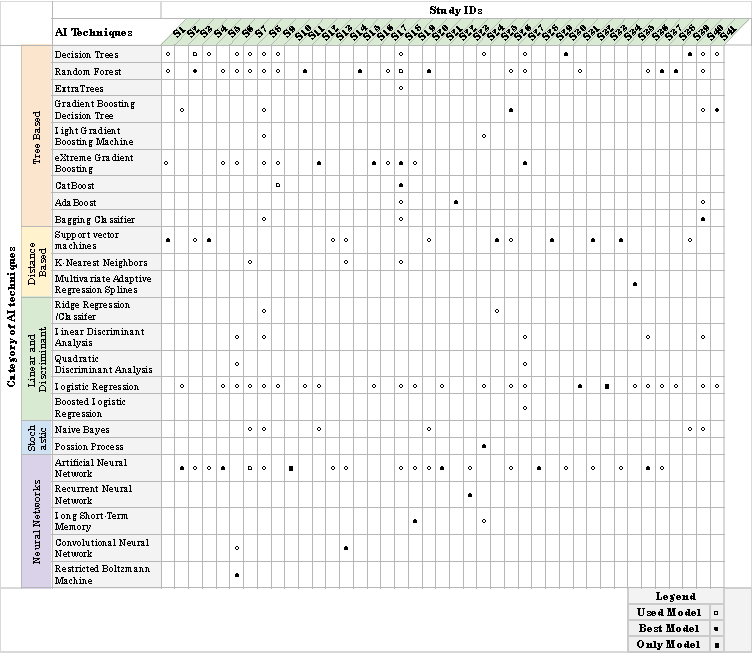
\includegraphics[width=\linewidth]{pdf_tables/results/RS_RQ4_techniques.pdf}
    %\vspace{-2.5cm}
\end{table}


\subsubsection{\RSRQfive}
\label{sec:RQ5}
Each application of AI typically requires a distinct set of evaluation metrics to effectively demonstrate and compare the performance of different algorithms, pre-processing methods, and training strategies. This is because the objectives and success criteria of AI tasks vary significantly between domains. A metric that may be highly informative in one context could be less meaningful or even misleading in another. This variability is particularly evident in churn prediction, where several specific factors influence metric selection. 
Our review of the 41 selected studies highlights these specific challenges. Firstly, churn datasets are often highly imbalanced, with churners representing only a small fraction of the total customer base. As a result, evaluation metrics that account for class imbalance are essential. Secondly, in practical business scenarios, marketing interventions aimed at reducing churn come at a cost. Therefore, it is often more critical to avoid misclassifying non-churners as churners (false positives) than to miss a few actual churners (false negatives). This cost-sensitive nature of churn prediction influences the choice and interpretation of performance metrics.

As shown in Table~\ref{table:metrics}, the most frequently used evaluation metrics across the selected studies include Accuracy, Precision, Recall, F1/F scores, and AUC-ROC. These metrics are particularly well-suited for assessing the performance of churn prediction algorithms. For example, Recall indicates the proportion of actual churners correctly identified by the model, while Precision reflects the proportion of predicted churners who are indeed true churners. These metrics are directly linked to the practical implications of false negatives and false positives, as discussed earlier. The F1 and F scores offer a harmonic mean of Precision and Recall, summarizing the model’s ability to balance these two aspects in a single value. In particular, the F score allows for adjustable weighting between Precision and Recall, providing flexibility to align the evaluation with specific business priorities. This makes it a valuable tool for deriving a single metric that captures both sensitivity and predictive accuracy. AUC-ROC is also widely used and regarded as a robust metric, especially in the context of class imbalance, which is common in churn prediction. It assesses the model’s ability to discriminate between churners and non-churners across all classification thresholds. In addition to these five commonly used metrics, several studies employ more specialized or domain-specific measures. These bespoke metrics are typically chosen to reflect particular research goals or business considerations of the authors.

\begin{table}[H]
    \centering
    \caption{Metrics to evaluate churn prediction techniques.}
    \label{table:metrics}
    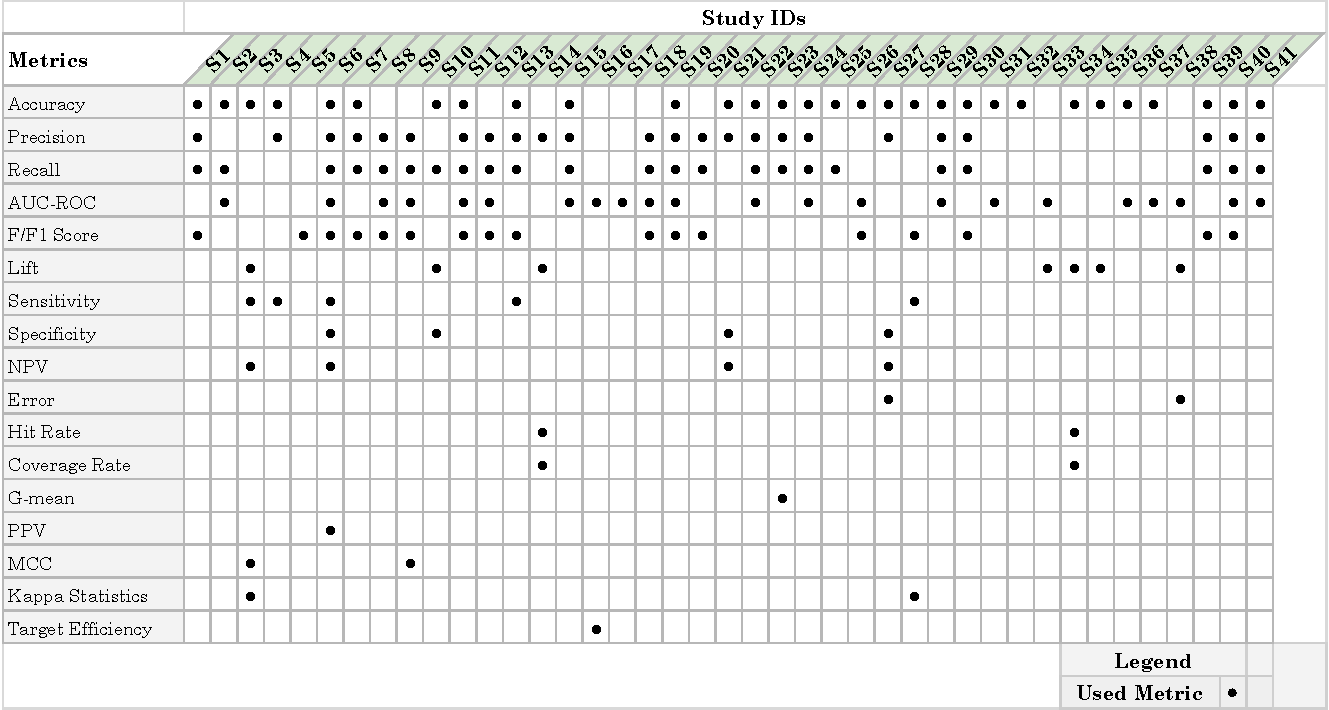
\includegraphics[width=\linewidth]{pdf_tables/results/RS_RQ5_metrics.pdf}
\end{table}


\subsubsection{\RSRQsix}
\label{sec:RQ6}
Very few papers provide a publicly available dataset (11 out of 41). However, it is still possible to find a diverse array of datasets employed for churn prediction in a non-contractual environment, having different contexts, data types, and business sectors. These datasets are primarily obtained from:
\begin{itemize}
    \item Open platforms such as Kaggle (e.g., the Retailrocket Recommender System Dataset \sid{D2} \cite{Dat2-verma2021ecommerce}, \sid{D4} \cite{Dat4-retailrocket2017dataset}, \sid{D5} \cite{Dat5-usmani2020pakistan}, \sid{D6} \cite{Dat6-regivm2021retail})
    \item Academic repositories (e.g., the Online Retail II dataset \sid{D3} \cite{Dat3-uci2021online}, \sid{D9} \cite{Dat9-recsyswiki2015grocery})
    \item Corporate contributions (e.g., the Brazilian E-Commerce Public Dataset by Olist \sid{D1} \cite{Dat1-olist2018brazilian}, \sid{D7} \cite{Dat7-dunnhumby2021source}, \sid{D8} \cite{Dat8-dunnhumby2021source})
\end{itemize}
\nocite{Dat1-olist2018brazilian, Dat2-verma2021ecommerce, Dat3-uci2021online, Dat4-retailrocket2017dataset, Dat5-usmani2020pakistan, Dat6-regivm2021retail, Dat7-dunnhumby2021source, Dat8-dunnhumby2021source, Dat9-recsyswiki2015grocery}

As illustrated in Table~\ref{table:available_datasets}, the datasets cover both online (E-Commerce) and offline (Brick-and-Mortar) scenarios and span multiple retail sectors, including merchandise, fashion, electronics, and food. These datasets differ not only in the retail sector they are related to, but also in structural characteristics, going from using only transactional records to multidimensional data including geo-demographic, behavioral, and interactional features. \\
It is interesting to note that the majority of the datasets are real-world datasets, but there is also a single synthetic dataset (i.e., the Retail Transaction Data) that is also used, showing attempts to simulate realistic churn behaviors for research purposes when actual data is limited or confidential. 

% DISCUSSION TOPIC? These synthetic datasets could be particularly useful for controlled experimentation and benchmarking if big and complex enough.
%is the following also a DISCUSSION TOPIC?
This research question clearly uncovered the difficulties associated with the churn prediction task: each business, sector, dataset, and even study set a different definition for churn (as seen in Section \ref{sec:RQ1}). This inherent feature of this problem creates difficulty in comparing frameworks (needing to be equal in not only the dataset, but also the churn definition), making it impossible in this review to make any kind of comparison.

The datasets that already provide a churn flag, stating whether the customer has churned or not, show insufficient documentation, i.e., it is impossible to trace back what the adopted definition of churn is. This impacts reproducibility and points to the need for greater transparency and standardization in data reporting. 
This review encourages the creation of a clear dataset description and the use of practices that can help future researchers better assess, compare, and build robust churn prediction models in the retail domain.

\begin{table}[h!]
\centering
\caption{Available datasets.}
\label{table:available_datasets}
%{\fontfamily{phv}\selectfont   % inizio gruppo → Helvetica/Arial-like
    \tiny                 % o \footnotesize, \small…
\resizebox{1\textwidth}{!}{
\begin{tabular}{
  |>{\centering\arraybackslash}p{0.1cm}
  |>{\centering\arraybackslash}p{1.8cm}
  |>{\centering\arraybackslash}p{0.7cm}
  |>{\centering\arraybackslash}p{1.3cm}
  |>{\centering\arraybackslash}p{1.3cm}
  |>{\centering\arraybackslash}p{1.1cm}
  |>{\centering\arraybackslash}p{2cm}
  |>{\centering\arraybackslash}p{1.8cm}
  |>{\centering\arraybackslash}p{0.7cm}
  |>{\centering\arraybackslash}p{0.7cm}
  |>{\centering\arraybackslash}p{0.7cm}
  |}
\hline
\rowcolor[HTML]{D9EAD3} 
      \multicolumn{1}{|c|}{\textbf{ID}}
      & \textbf{Dataset name}
      & \textbf{\begin{tabular}[c]{@{}c@{}}Pub.\\year\end{tabular}}
      & \textbf{\begin{tabular}[c]{@{}c@{}}Retail\\sector\end{tabular}}
      & \textbf{\begin{tabular}[c]{@{}c@{}}Synthetic/\\Real\end{tabular}}
      & \textbf{\begin{tabular}[c]{@{}c@{}}Online/\\Physical\end{tabular}}
      & \textbf{\begin{tabular}[c]{@{}c@{}}Features\\categories\end{tabular}}
      & \textbf{\begin{tabular}[c]{@{}c@{}}Dataset\\size\end{tabular}}
      & \textbf{\begin{tabular}[c]{@{}c@{}}Churn\\Flag\end{tabular}}
      & \textbf{\begin{tabular}[c]{@{}c@{}}Churn\\Rate\end{tabular}}
      & \textbf{\begin{tabular}[c]{@{}c@{}}Study\\IDs\end{tabular}}\\ \hline
\multicolumn{1}{|c|}{\sid{D1}} & \begin{tabular}[c]{@{}c@{}}Brazilian \\ e-commerce \\ public dataset \\ by Olist \\ \cite{Dat1-olist2018brazilian}\end{tabular} & 2018 & \begin{tabular}[c]{@{}c@{}}fashion, \\ mobile, \\ electronics, \\ appliance, \\ etc.\end{tabular} & Real & Online & Transactional & \# Orders: 100k & F & NA & \begin{tabular}[c]{@{}c@{}}S3,\\ S5,\\S10,\\ S20\end{tabular} \\ \hline
\sid{D2} & \begin{tabular}[c]{@{}c@{}}E-commerce \\ customer \\ churn analysis \\ and prediction \\ \cite{Dat2-verma2021ecommerce}\end{tabular} & 2021 & NA & NA & Online & \begin{tabular}[c]{@{}c@{}}Geodemographic, \\ Demographic,\\ Behavioural,\\ Transactional,\\ Interactional\end{tabular} & \# Rows: 5630 & T & 20.24\% & S7 \\ \hline
\sid{D3} & Online Retail II \cite{Dat3-uci2021online}& 2012 & gift-ware & Real & Online & Transactional & \begin{tabular}[c]{@{}c@{}}\# Instances: \\ 1,067M\end{tabular} & F & NA & S5, S8 \\ \hline
\sid{D4} & \begin{tabular}[c]{@{}c@{}}Retailrocket \\ recommender\\  system dataset \\ \cite{Dat4-retailrocket2017dataset}\end{tabular} & 2022 & \begin{tabular}[c]{@{}c@{}}fashion, \\ mobile, \\ electronics, \\ appliance, \\ etc\end{tabular} & Real & Online & \begin{tabular}[c]{@{}c@{}}Behavioural, \\ Transactional\end{tabular} & \begin{tabular}[c]{@{}c@{}}\# Events: 2,7M\\ \# Unique \\ Visitors: 1,4M\\ \# Product \\ Information: \\ 20M\\ \# Unique Items: \\ 417k\end{tabular} & F & NA & S26, S29 \\ \hline
\sid{D5} & \begin{tabular}[c]{@{}c@{}}Pakistan's \\ largest \\ e-commerce \\ dataset \\ \cite{Dat5-usmani2020pakistan}\end{tabular} & \begin{tabular}[c]{@{}c@{}}2020/\\ 2021\end{tabular} & \begin{tabular}[c]{@{}c@{}}fashion, \\ mobile, \\ electronics, \\ appliance, \\ etc.\end{tabular} & Real & Online & Transactional & \begin{tabular}[c]{@{}c@{}}\# Transactions: \\ 500K\end{tabular} & F & NA & S8 \\ \hline
\sid{D6} & \begin{tabular}[c]{@{}c@{}}Retail \\ Transaction \\ Data \\ \cite{Dat6-regivm2021retail}\end{tabular} & \begin{tabular}[c]{@{}c@{}}2017/\\ 2018\end{tabular} & NA & Synthetic & NA & Transactional & \begin{tabular}[c]{@{}c@{}}\# Transactions: \\ 125K\end{tabular} & F & NA & S25 \\ \hline
\sid{D7} & Carbo-loading \cite{Dat7-dunnhumby2021source} & \begin{tabular}[c]{@{}c@{}}Last \\ update: \\ 2023\end{tabular} & Food & Real & \begin{tabular}[c]{@{}c@{}}Offline \\ (Brick and \\ Mortar)\end{tabular} & NA & \begin{tabular}[c]{@{}c@{}}\# Transactions: \\ 5M+\end{tabular} & F & NA & S24 \\ \hline
\sid{D8} & \begin{tabular}[c]{@{}c@{}}The complete \\ journey \\ \cite{Dat8-dunnhumby2021source} \end{tabular} & NA & Food & Real & \begin{tabular}[c]{@{}c@{}}Offline \\ (Brick and \\ Mortar)\end{tabular} & NA & \begin{tabular}[c]{@{}c@{}}\# Transactions: \\ 10M+\end{tabular} & F & NA & S24 \\ \hline
\sid{D9} & A-feng dataset \cite{Dat9-recsyswiki2015grocery} & \begin{tabular}[c]{@{}c@{}}Last\\ update: \\ 2015\end{tabular} & Food & Real & \begin{tabular}[c]{@{}c@{}}Offline \\ (Brick and \\ Mortar)\end{tabular} & \begin{tabular}[c]{@{}c@{}}Geodemographic, \\ Demographic, \\ Transactional\end{tabular} & \begin{tabular}[c]{@{}c@{}}\# Transactions: \\ 817K\\ \# Users: 32k\\ \# Items: 23,8K\end{tabular} & NA & NA & S28 \\ \hline
\end{tabular}
}
%  }% fine gruppo → torna al font normale qui
\end{table}
\FloatBarrier

\subsubsection{\RSRQseven}
\label{sec:RQ7}
%\DD{}{A list of citations is followed by a period or comma, not the other way around. Correct.}

Fifteen of the 41 selected studies explicitly discuss challenges and limitations encountered in their research. These can be broadly categorized into five groups, as shown in Table \ref{tab:PS_RQ_7_Challenges_and_limitations}. A detailed description of the categories is provided below.


\begin{itemize}
    \item \textit{Data availability:} Datasets used to experiment with methods for customer churn prediction are often limited in size, synthetic, or come from a single retailer or business sector. Incorporating data from multiple sectors and/or retailers could help build more resilient models and uncover deeper behavioral patterns.

    \item \textit{Domain limitation:} This issue is closely linked to data availability and highlights the lack of data sources from diverse business domains. Much of the research on customer churn prediction is focused exclusively on either online or offline retail contexts, making it difficult to transfer findings or techniques across channels. Since customer dynamics can vary significantly across sectors, a domain-independent model needs to be trained on data with sufficient domain diversity to ensure generalizability.

    \item \textit{Lack of comparative frameworks:} This issue emphasizes the absence of comprehensive testing and comparisons across a broad spectrum of AI frameworks and techniques. Without such comparisons, it is difficult to draw reliable conclusions regarding the relative performance of different approaches for churn prediction.

    \item \textit{Computational resource limitation:} This issue pertains to constraints in computational resources available to researchers. Limited computational power prevents the exploration of optimal hyper-parameter configurations and restricts the ability to test larger or more complex models on substantial datasets, potentially limiting the performance and scalability of the proposed techniques.

    \item \textit{Lack of robustness:} This issue concerns instances where technical inconsistencies arise, such as results that contradict the researchers’ hypotheses or the presence of known weaknesses in the employed models that may introduce bias or skew results, undermining their theoretical validity.
\end{itemize}

\begin{table}[h]
\caption{Challenges and limitations presented in the reviewed studies.}
\label{tab:PS_RQ_7_Challenges_and_limitations}
\centering
\scriptsize
\resizebox{0.9\textwidth}{!}{
\begin{tabular}{|
>{\centering\arraybackslash}m{5cm}
|>{\centering\arraybackslash}m{8cm}|}
\hline
\rowcolor[HTML]{D5E8D4}
\rule[-1.5ex]{0pt}{4ex}\textbf{Challenges and Limitations}
& \rule[-1.5ex]{0pt}{4ex}\textbf{Study IDs} \\ \hline
Data availability & S4, S16, S21, S28, S31, S36, S37, S38 \\ \hline
Domain limitation & S4, S15, S29, S30, S31, S33, S37 \\ \hline
Lack of comparative frameworks & S16, S22, S23, S30 \\ \hline
Computational resource limitation & S15, S22 \\ \hline
Lack of robustness & S9, S38  \\ \hline
\end{tabular}
}
\end{table}


\begin{comment}
%Out of the 41 studies selected, 15 explicitly discussed the challenges faced in their research. 
The most prominent concern raised by the selected studies is data availability: datasets are often limited in size, synthetic, or come from a single retailer or sector. Incorporating data from multiple sectors and/or retailers could help build more resilient models and uncover deeper behavioral patterns \cite{S4-ID40-Barzegar, S16-ID325-Matuszelanski, S19-ID363-Agbemadon, S20-ID379-Baghla, S21-ID389-Seymen, S30-ID647-Rachid, S31-ID717-Migueis, S33-ID742-Migueis, S36-ID806-Ching, S37-ID826-Buckinx}.

Another challenge raised by the studies is linked to domain limitations. It is pointed out that much of the research on customer churn prediction is focused exclusively on either online or offline retail contexts, making it difficult to transfer findings or techniques across channels \cite{S4-ID40-Barzegar, S16-ID325-Matuszelanski, S30-ID647-Rachid, S31-ID717-Migueis, S33-ID742-Migueis, S37-ID826-Buckinx}.

The narrow model diversity is also pointed out by the authors, where they highlight that most works rely on a limited set of algorithms, often lacking in comparative analysis with more recent or diverse AI techniques. This lack of methodological breadth can make it harder to identify the best-performing approaches \cite{S16-ID325-Matuszelanski, S22-ID394-Wu, S30-ID647-Rachid}.

Some studies also point out that the computational costs are a common performance bottleneck. Processes such as grid search for hyperparameter tuning are rarely performed exhaustively, which may prevent models from reaching their optimal performance. The studies have cited the computational constraints as a reason behind not being able to fully explore the parameter space \cite{S15-ID297-Georgiou, S22-ID394-Wu, S38-ID833-Burez, S29-ID538-Berger}.
Therefore, when comparing different techniques, the observed performance may not reflect each method's full potential.
%, as resource constraints can limit the ability to optimize hyper-parameters effectively for each method.
Another limitation raised is related to the methodological assumptions and experimental design. For instance, some clustering approaches failed to meet variance assumptions, undermining their theoretical validity. In several cases, a lack of rigorous evaluation protocols was reported, raising questions about the robustness and reproducibility of the findings \cite{S9-ID95-Coolwijk, S23-ID396-Pondel, S38-ID833-Burez}.
\end{comment}

\subsubsection{\RSRQeight}
\label{sec:RQ8}
Of the 41 selected studies, 31 provided directions for future research. The proposed directions can be broadly grouped into seven categories which can be observed in Table \ref{tab:PS_RQ_8_Future_directions}. The details of the categories are as follows:

\begin{itemize}

    \item \textit{Exploring new frameworks:} Studies in this category suggest employing a broader range of AI techniques and fully exploiting these methods through hyperparameter tuning and architectural optimizations. The utilization of more advanced architectures, such as Recurrent Neural Networks, ensemble learning, transformers, and hybrid models combining supervised and unsupervised techniques, is expected to better capture sequential dependencies, rare events, and subtle patterns in customer behavior, potentially improving churn prediction performance. Additionally, to fully exploit the capabilities of AI models, studies propose optimization efforts, including hyperparameter tuning and dynamic adaptation to concept drift, which is gaining increasing attention. Techniques such as online learning, adaptive algorithms, and automated feature engineering pipelines are suggested to better handle evolving customer behaviors and seasonal trends.


    \item \textit{Data and domain augmentation:} Studies in this category propose integrating richer and more diverse data sources, including social media sentiment, transactional history, weather patterns, spatial data, and socio-economic indicators. Together, these sources can offer a more holistic view of customer behavior and improve the generalizability of predictive models across various contexts. Furthermore, incorporating data from different retail sectors, such as fashion, electronics, and others, can enhance generalizability by ensuring that datasets capture a wider range of customer behaviors, which often vary between domains.
    
    \item \textit{Customer segmentation and behavioral features:} Proposals in this category are similar to data augmentation efforts but focus specifically on incorporating behavioral features, such as web navigational data from e-commerce or hybrid retailers. Furthermore, some studies propose deriving intermediate features, such as customer segments, and providing this information to AI models to offer additional context about customers.
    
    \item \textit{Temporal dynamics:} Studies in this category propose techniques aimed at more effectively capturing and leveraging the temporal dynamics of data. Such proposals include utilizing time series data directly, as well as exploring methods that allow models to better capture time-based patterns, such as experimenting with different window lengths and time series scales.
    

    \item \textit{Explainability:} Studies propose techniques to improve the interpretability of AI models. This includes understanding the relative importance of various features by using tools such as Shapley values. Improving AI model explainability can foster greater trust in the models and provide deeper insights into the complex reasons behind customer churn.

    \item \textit{ROI impact:} Studies emphasize considering the return on investment (ROI) implications when evaluating churn prediction models. For example, falsely predicting a non-churner as a churner has a higher negative financial impact than failing to identify a potential churner, as promotional resources would be wasted in the former case.
    
    \item \textit{Real-world deployment:} Studies propose validating customer churn prediction models in real-world environments. Such validation would not only help assess churn prediction performance but also reveal the actual financial impact on businesses when these systems are integrated into promotional campaigns.
    
\end{itemize}

\begin{table}[H]
\caption{Future directions presented in the reviewed studies.}
\label{tab:PS_RQ_8_Future_directions}
\centering
\scriptsize
\resizebox{0.9\textwidth}{!}{
\begin{tabular}{|
>{\centering\arraybackslash}m{5cm}
|>{\centering\arraybackslash}m{8cm}|}
\hline
\rowcolor[HTML]{D5E8D4}
\rule[-1.5ex]{0pt}{4ex}\textbf{Future directions}
& \rule[-1.5ex]{0pt}{4ex}\textbf{Study IDs} \\ \hline
Exploring new frameworks & S3, S4, S5, S6, S7, S9, S10, S11, S13, S14, S18, S19, S20, S22, S23, S24, S25, S26, S28, S30, S33, S38, S41 \\ \hline
Data \& domain augmentation & S2, S3, S4, S7, S10, S11, S16, S19, S20, S21, S22, S26, S30, S31, S33, S36, S37 \\ \hline
Customer segmentation and behavioral features & S6, S14, S15, S16, S21, S22, S28, S30, S33 \\ \hline
Temporal dynamics & S4, S5, S15, S21, S23, S24, S31, S36 \\ \hline
Explainability & S5, S7, S26, S41  \\ \hline
ROI impact & S3, S12, S15, S37 \\ \hline
Real-world deployment & S2, S14 \\ \hline
\end{tabular}
}
\end{table}

%Approximately three quarters of the selected studies offered insights into future research directions, revealing a growing consensus on how to improve customer churn prediction using AI techniques. 
\begin{comment}
    
Several of the 41 studies analyzed propose future research directions, revealing a growing consensus on how to improve Customer Churn Prediction using AI techniques. One key area involves the integration of richer and more diverse data sources, including social media sentiment, transactional history, weather patterns, spatial data, and socio-economic indicators, which together can offer a more holistic view of customer behavior and improve the generalizability of predictive models across contexts \cite{S3-ID223-Beckhauser,S11-D105-Sunarya,S16-ID325-Matuszelanski,S19-ID363-Agbemadon}.

Another promising direction is the improvement of feature engineering and segmentation strategies, through techniques such as signal transformation, wrapper selection, or behavioral clustering. These methods extract meaningful patterns from complex datasets, particularly regarding temporal dynamics or customer lifecycle transitions \cite{S3-ID223-Beckhauser,S9-ID95-Coolwijk,S15-ID297-Georgiou,S21-ID389-Seymen,S23-ID396-Pondel}.

Researchers also highlight the need for developing explainable AI models, particularly deep learning architectures that incorporate intrinsic attention mechanisms or Shapley interpretability tools. This could improve both stakeholder trust and diagnostic capabilities in business settings \cite{S5-ID50-Pasquadibisceglie,S7-ID79-Boukrouh,S26-ID442-Fridrich}.

Another direction is the automation of model optimization, including hyperparameter tuning and dynamic adaptation to concept drift, which is gaining increasing attention. Several studies propose leveraging techniques like online learning, adaptive algorithms, and automated feature pipelines to handle evolving customer behaviors and seasonal trends more effectively \cite{S5-ID50-Pasquadibisceglie,S26-ID442-Fridrich}.

There is also increasing interest in advanced architectures, such as Recurrent Neural Networks (RNNs), ensemble learning, transformers, and hybrid models combining supervised and unsupervised techniques. These models are seen as more capable of capturing sequential dependencies, rare events, or subtle patterns in customer behavior (e.g., partial vs. full churn) \cite{S6-ID70-Mahdi,S10-ID98-Seema,S13-ID202-Gangadhar,S14-ID226-Seymen,S20-ID379-Baghla}.
Several studies also point to the importance of real-world deployment, calling for more work on scalability and the development of web-based decision-support tools \cite{S2-ID16-Lu,S14-ID226-Seymen}.

Additionally, future work is expected to examine cost-benefit trade-offs, incorporating profitability metrics, customer lifetime value, and ROI assessments into churn modeling pipelines \cite{S12-ID198-Tuo,S15-ID297-Georgiou}.
Moreover, multiple authors advocate for creating publicly available benchmark datasets and standardized evaluation protocols to facilitate direct comparison of churn prediction approaches and foster reproducibility across the field \cite{S3-ID223-Beckhauser}.

Finally, a noteworthy emerging area is the spatial and temporal dimension of churn. Authors encourage the use of geospatial analysis, segment evolution tracking, and time-window sensitivity to better capture customer behaviors in both physical and digital environments, especially in hybrid retail ecosystems \cite{S16-ID325-Matuszelanski,S24-ID414-Zheng}.
\end{comment}